\chapter{\label{chap:entwurf}Konzeption}
Die erarbeiteten Anforderungen an ein Ampelinformationssystem für FahrradfahrerInnen werden in diesem Kapitel für die Konzeption angewendet. Beginnend mit dem Aufbau der Anwendung werden in den folgenden Abschnitten das Design, die von der Anwendung genutzten Daten, Anwendungsfälle, die Architektur und schließlich die Komponenten der Entwicklumgsumgebung, welche eingesetzt werden aufgeführt. 
\section{Anwendungsaufbau}
Android. \\ Activities bzw 1 Activity. \\ Action Bar / Einstellungen? \\
% ### Design ###
\section{Das Design}
Aus den Anforderungen an die graphische Oberfläche in Kapitel \ref{chap:anforderungen} entsteht das Design. Durch die überschaubare Anzahl an Funktionalitäten kann der Aufbau einfach gehalten werden. Aus den Empfehlungsanzeigen, welche den Systemzuständen entsprechen sind vier Fenster abzuleiten. Die folgende Abbildung zeigt den Entwurf der Benutzeroberfläche. \\
Abbildung \ref{fig:stop} zeigt die grapfische Umsetzung des Zustands \textit{a}, in dem die Ampelschaltung keine Weiterfahrt ermöglicht. Es wird ein großer roter Kreis mit einem schwarzen Kreuz verwendet. Rot ist eine Signalfarbe und steht auch bei Ampeln für "'Halt"' oder "'Stop"'. Auch das Kreuz wird häufig als \textit{verweigerndes} Symbol eingesetzt und ist somit intuitiv als solches erkennbar.\\
Abbildung \ref{fig:yeah} setzt die Visualisierung des Zustands \textit{b} um, bei dem man mit der aktuellen Geschwindigkeit in der Grünen Welle mitschwimmt, um. Hier wird ist ein großer grüner Kreis verwendet, in der Mitte steht "'ok"'. Durch die nicht alleinige Benutzung der Ampelfarben Rot und Grün ist die Ansicht auch für Menschen mit einer Rot-Grün-Sehschwäche eindeutig interpretierbar.\\
Die Abbildungen \ref{fig:langsamer} und \ref{fig:schneller} für die Zustände \textit{c} und \textit{d} sind in der Anordnung der Elemente identisch. Mittig im Bild ist eine eingekreiste rote Zahl die den Countdown der Restrotanzeige darstellt. Sie wird also mit jeder Sekunde aktualisiert. Ober- und unterhalb des Countdowns befinden sich jeweils zwei hellblaue Pfeile. Je nach Differenz der aktuellen zur berechneten Geschwindigkeit sind ein oder zwei Pfeile ausgefüllt. Wird also empfohlen viel schneller zu fahren, sind die oberen Pfeile aktiv, bei der Aufforderung etwas das Tempo zu drosseln der untere. Als Farbe für die Pfeile wurde Hellblau gewählt. Sie unterscheidet sich sowohl farblich als auch in der Helligkeitsstufe zu den anderen Farben und steht im hohen Kontrast zu dem Hintergrund. Auf schwarzem Hintergrund wirken die Farben intensiver und sind so auch aus dem Augenwinkel leichter zu erkennen und unterscheiden. 
\begin{figure}[H]
        \centering
           \begin{subfigure}[t]{0.23\textwidth}
                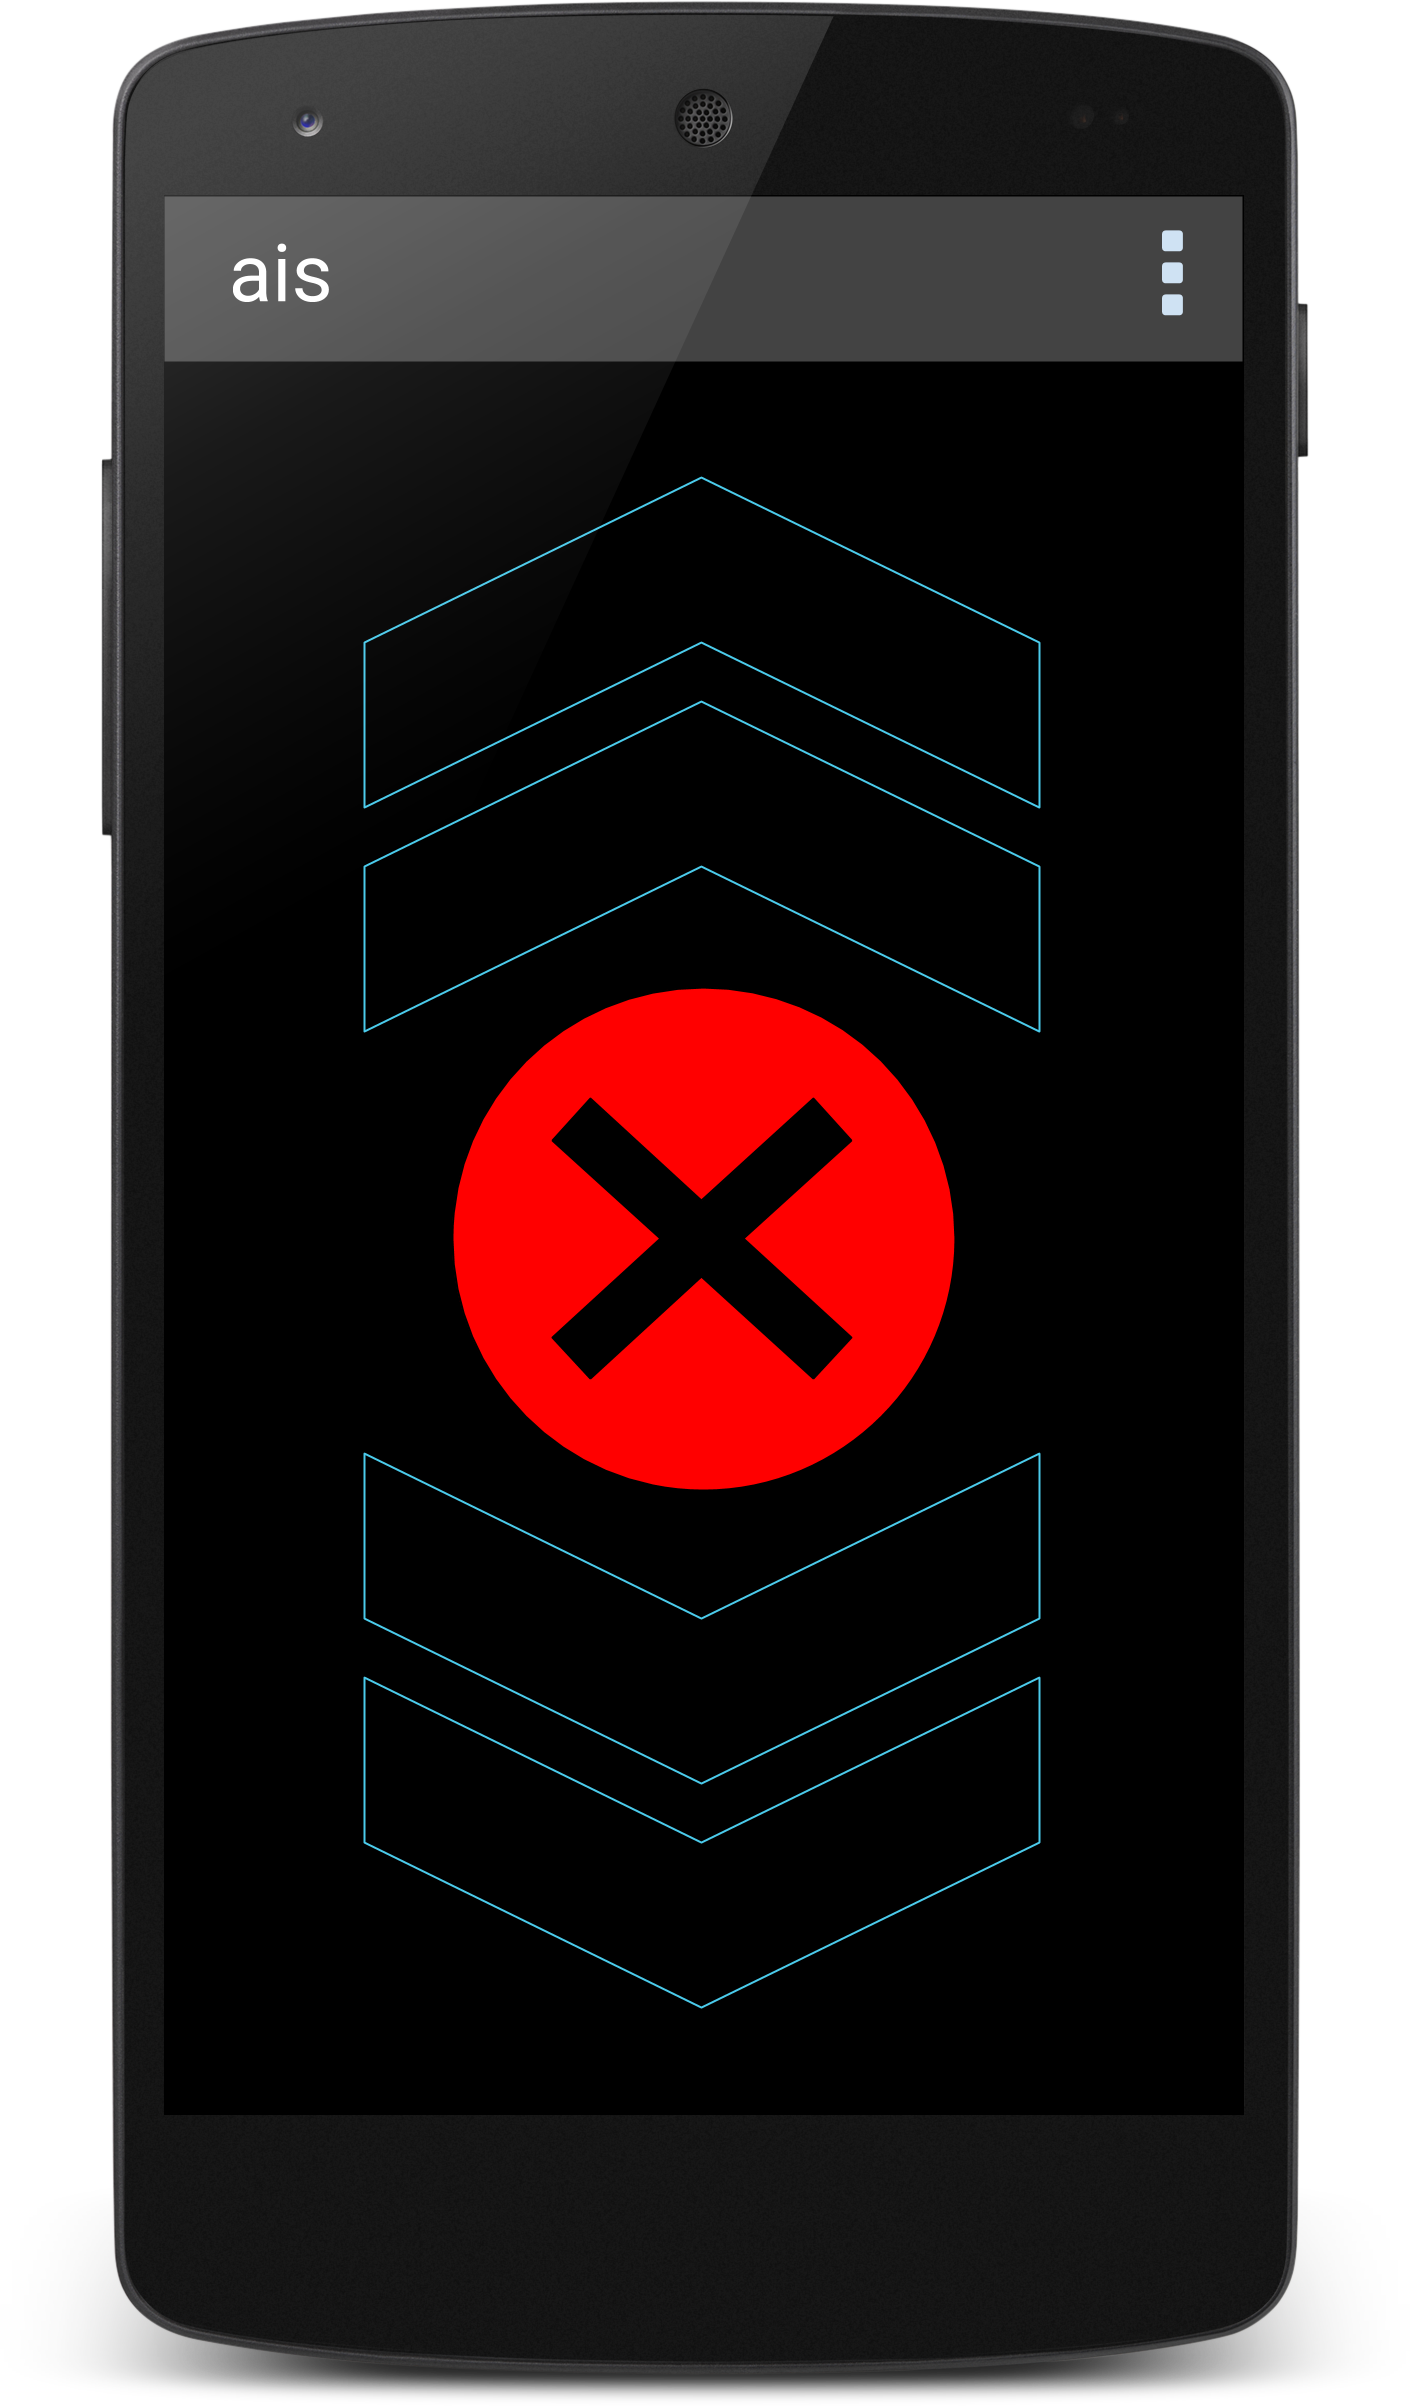
\includegraphics[width=\textwidth]{stop}
                \caption[Systemzustand a]{keine Weiterfahrt möglich}
                \label{fig:stop}
        \end{subfigure}
           ~ 
              \begin{subfigure}[t]{0.23\textwidth}
                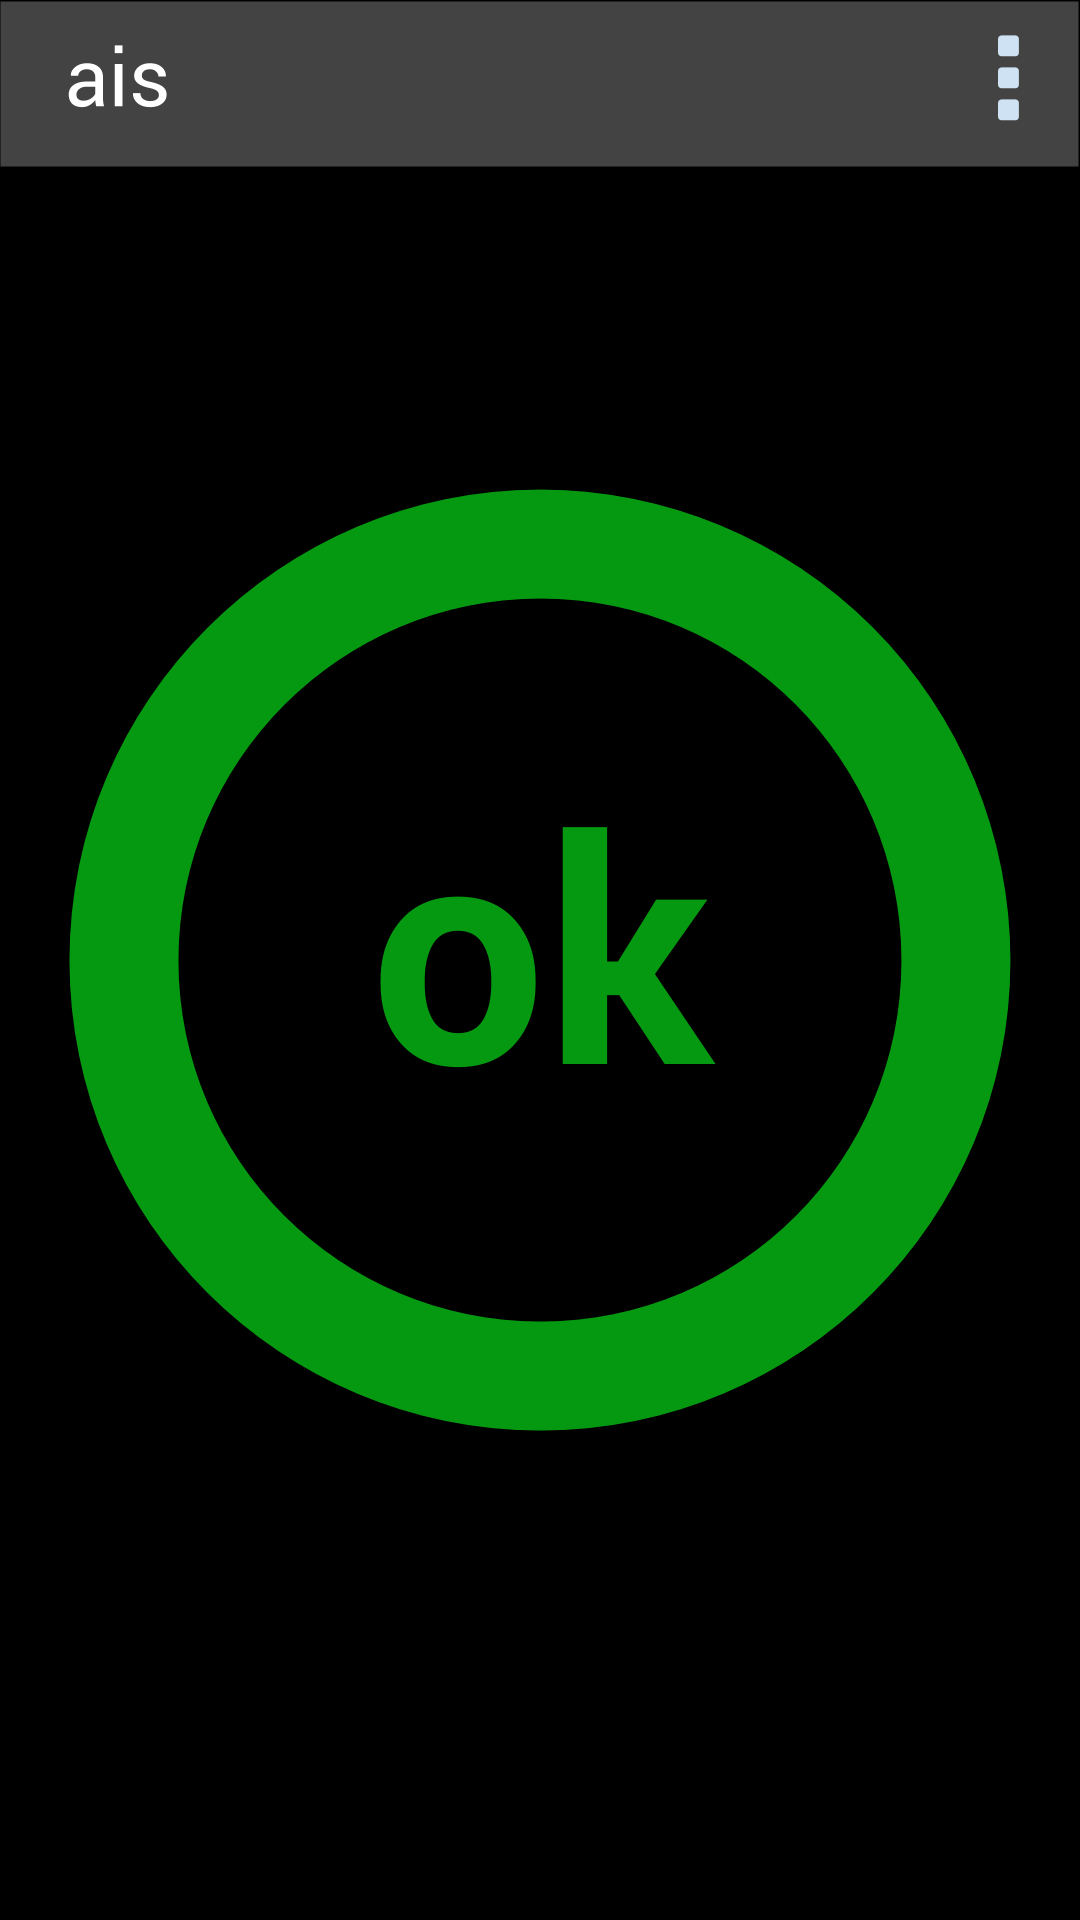
\includegraphics[width=\textwidth]{yeah}
                \caption[Systemzustand b]{Kein Aktionsbedarf}
                \label{fig:yeah}
        \end{subfigure}
           ~
        \begin{subfigure}[t]{0.23\textwidth}
                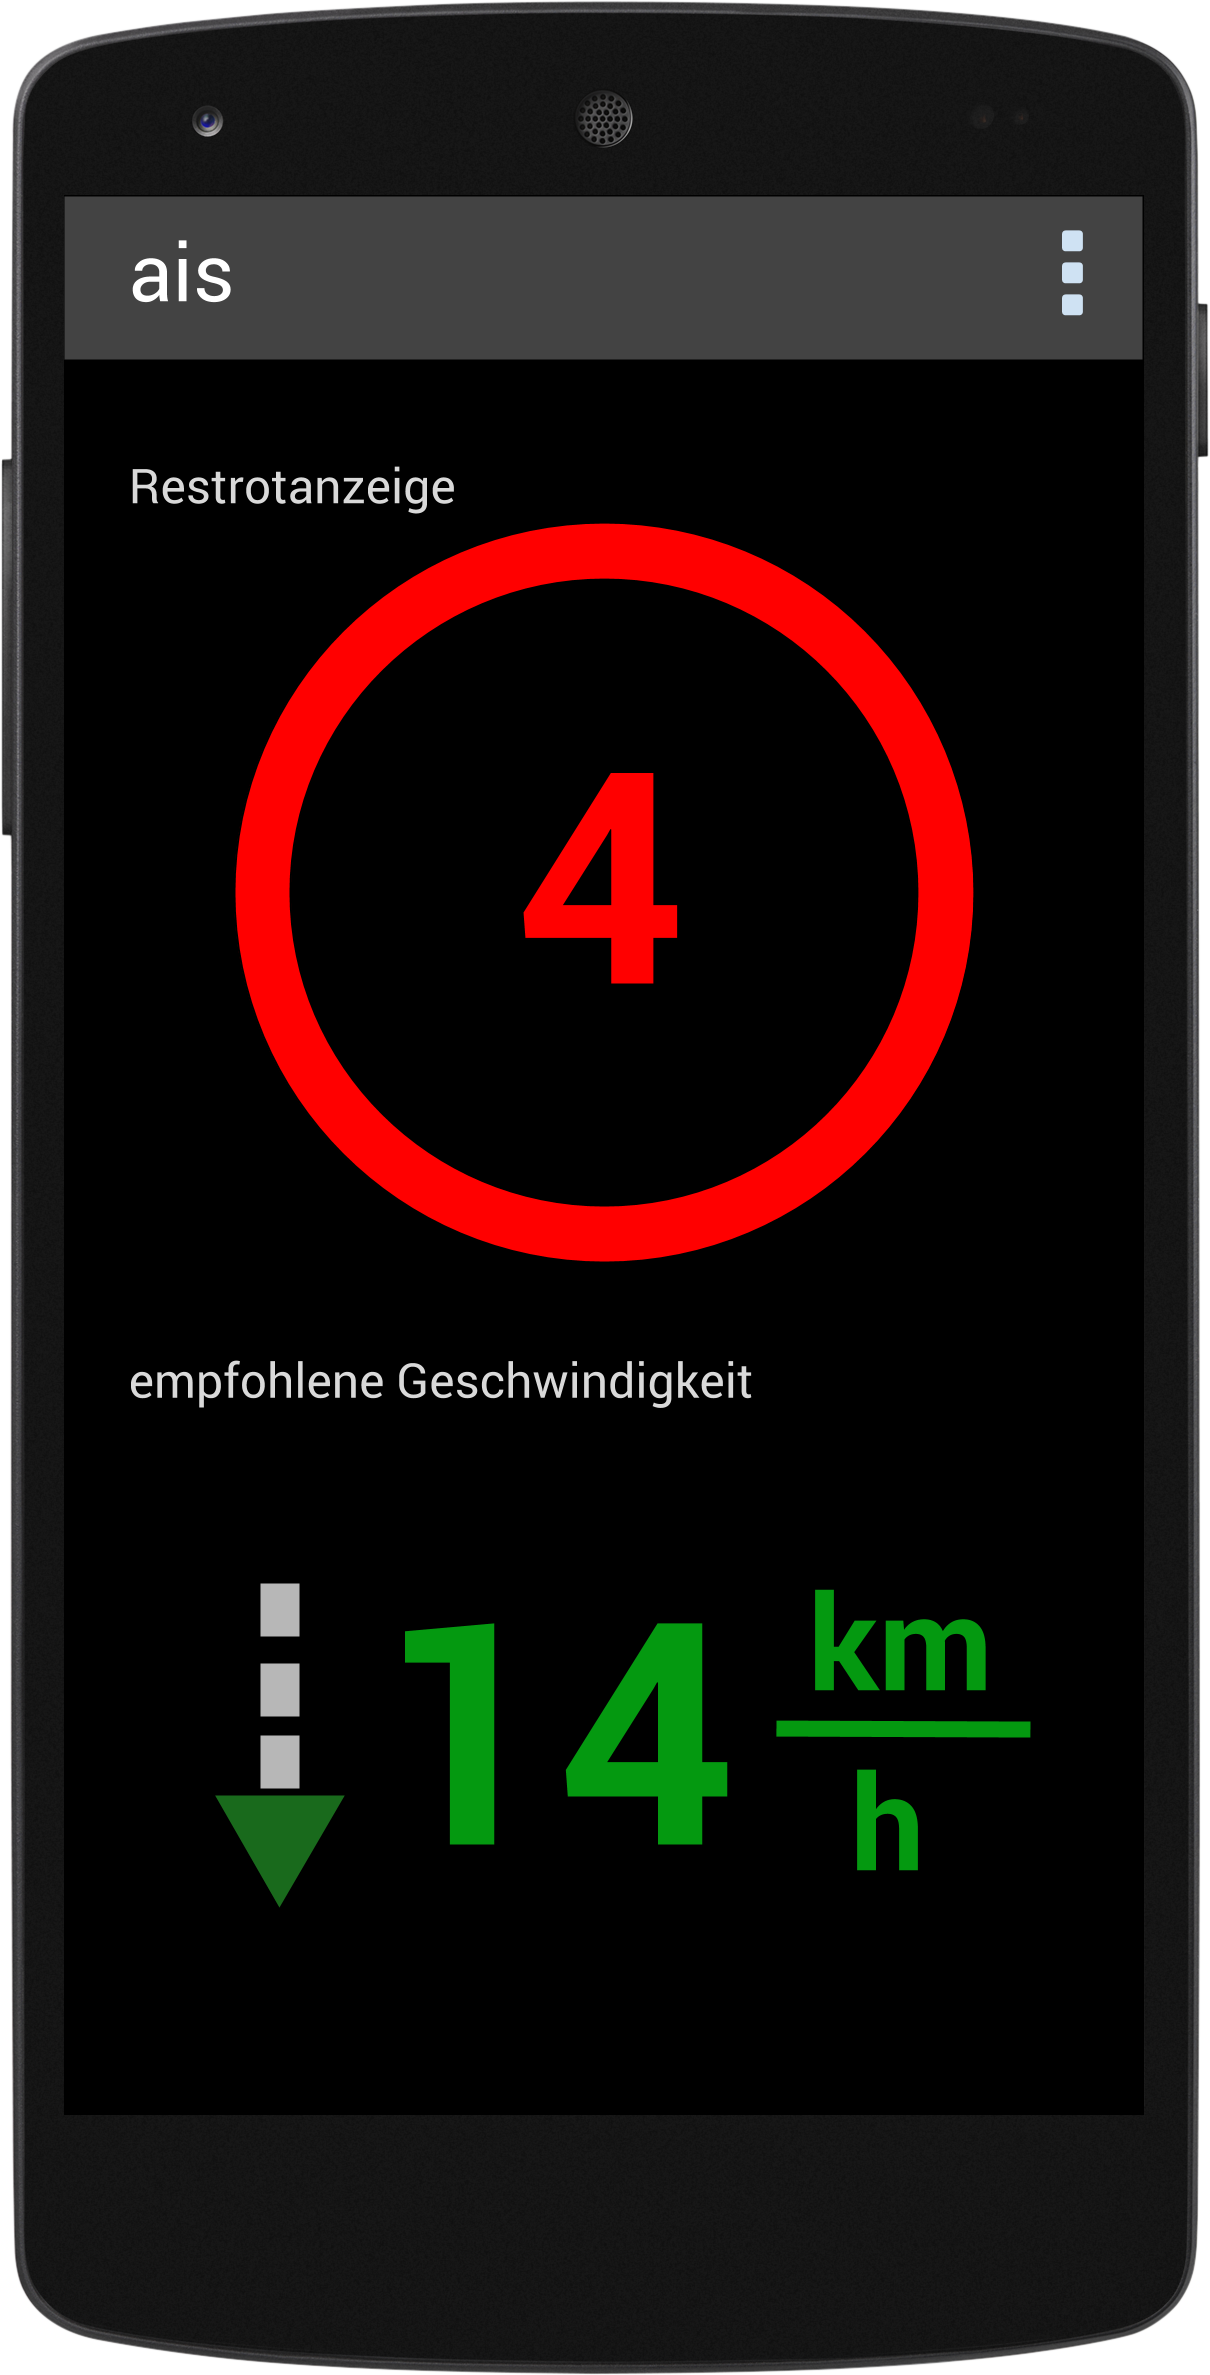
\includegraphics[width=\textwidth]{langsamer}
                \caption[Systemzustand c]{Weiterfahrt durch Verlangsamung  möglich}
                \label{fig:langsamer}
        \end{subfigure}
        ~
        \begin{subfigure}[t]{0.23\textwidth}
                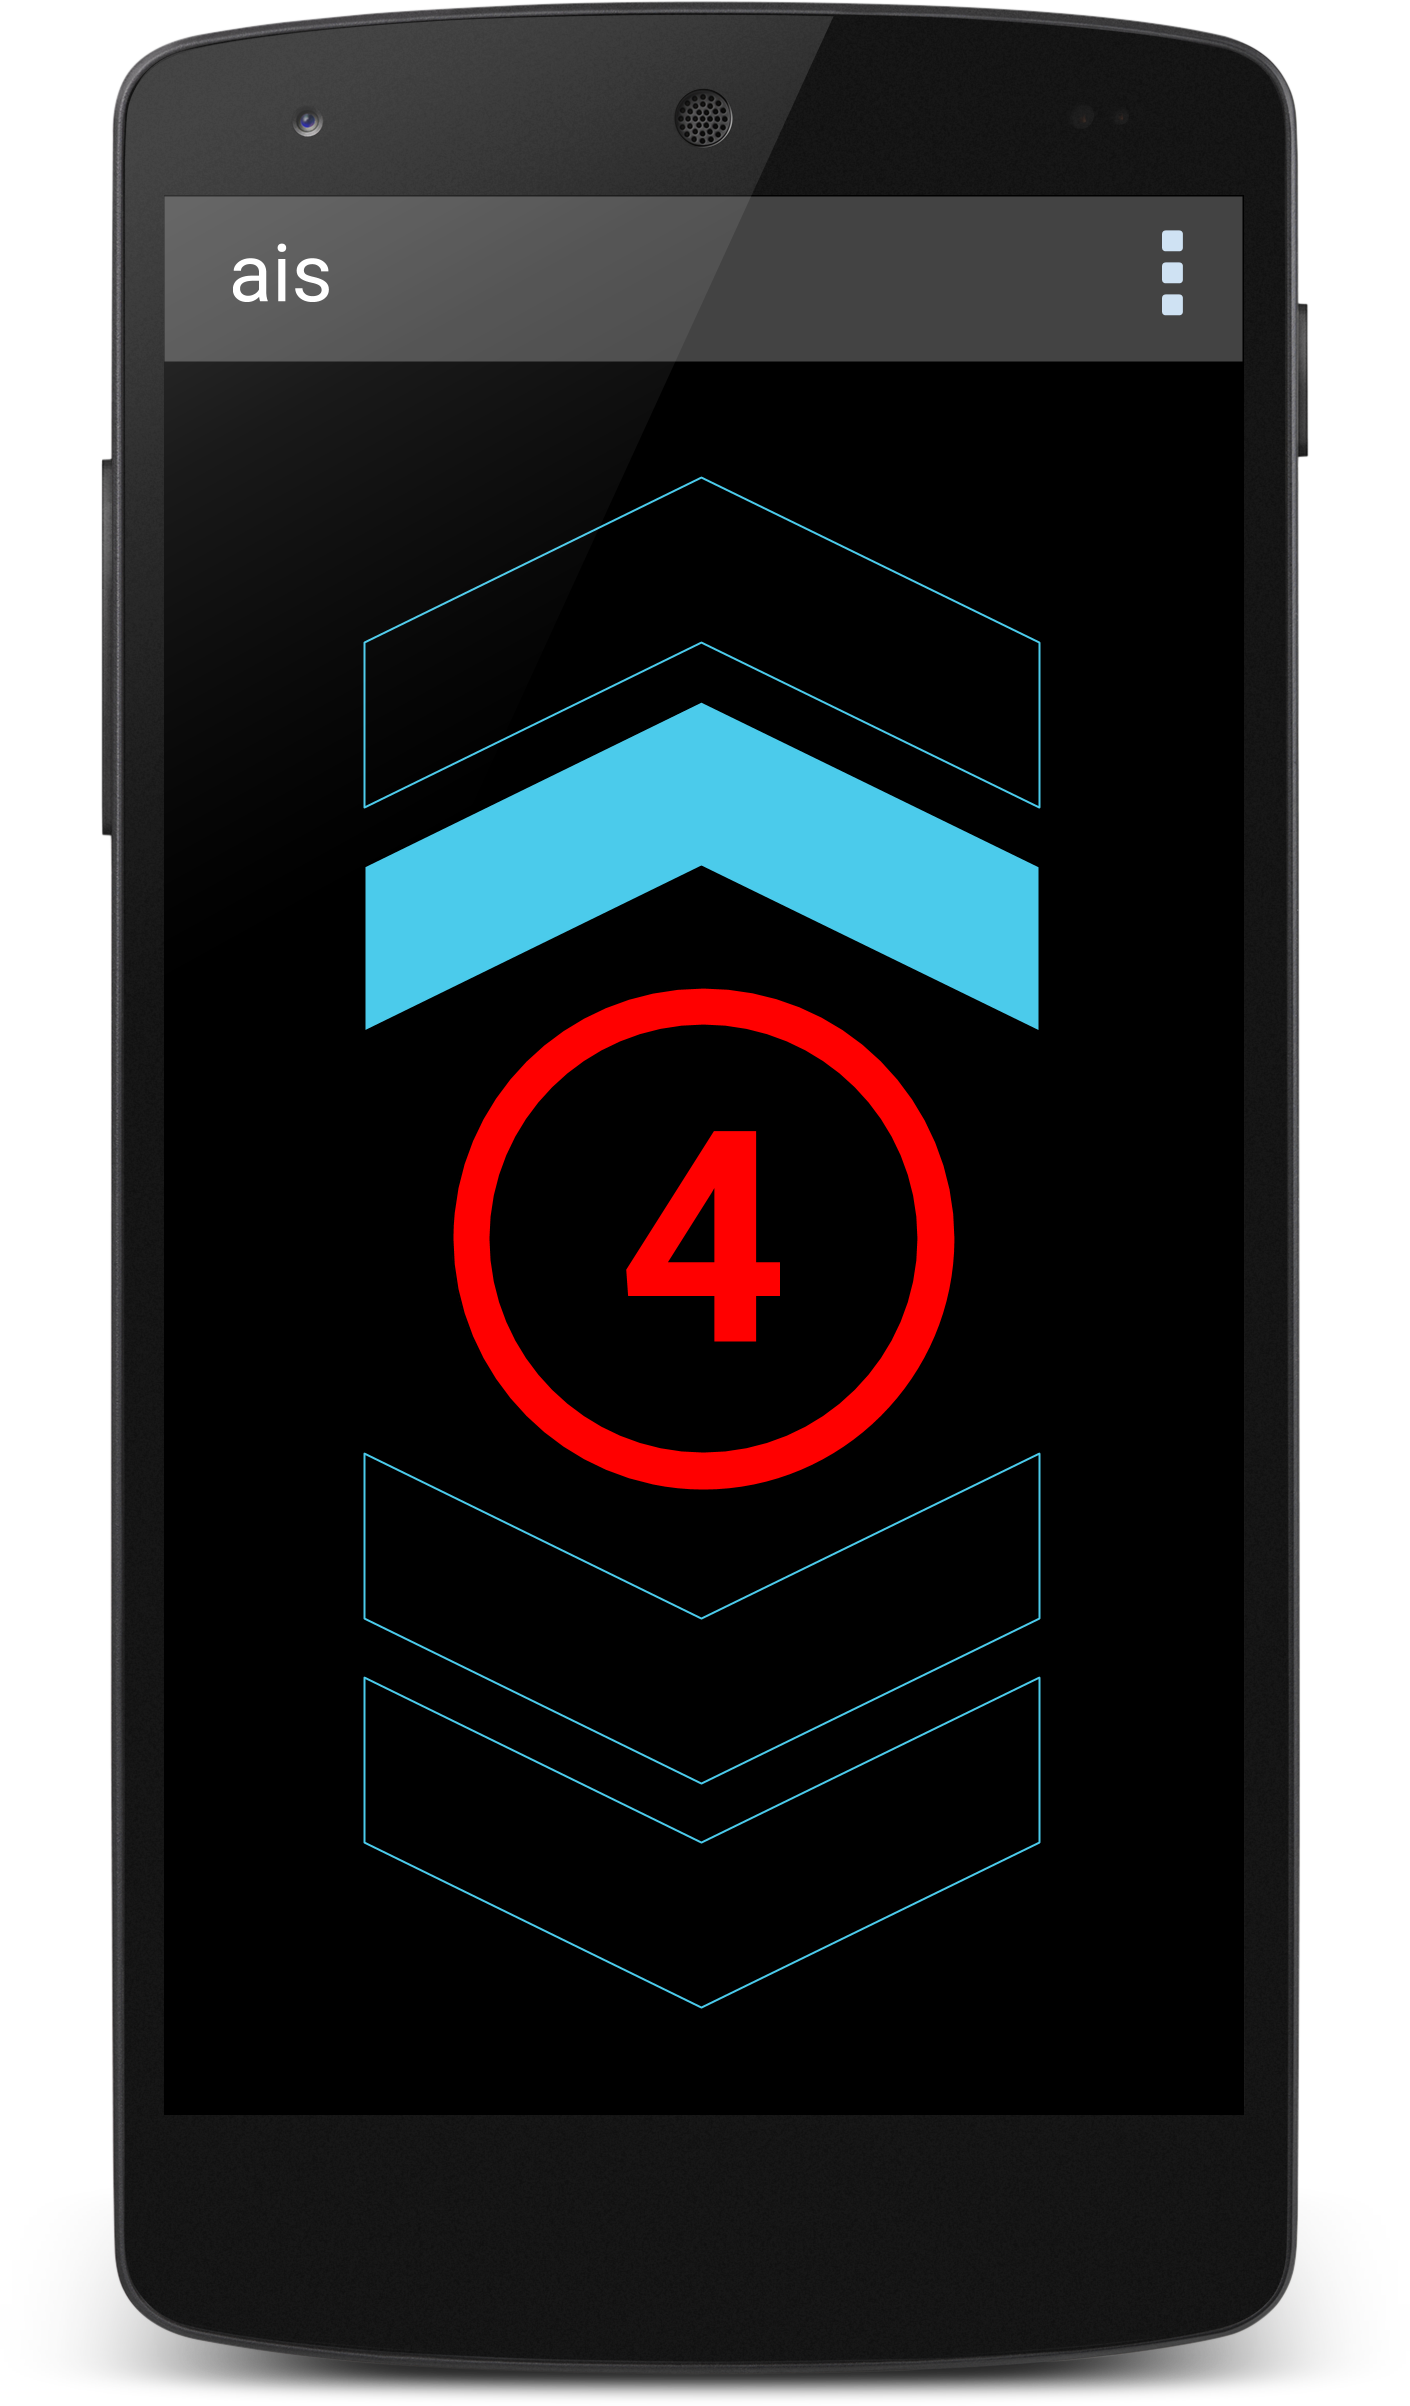
\includegraphics[width=\textwidth]{schneller}
                \caption[Systemzustand d]{Weiterfahrt durch Beschleunigung möglich}
                \label{fig:schneller}
        \end{subfigure}     
        \caption[Systemzustände im Ampelbereich]{Entwurf des Designs anhand der Systemzustände}
        \label{fig:mockup}
\end{figure} 
Die aktuelle Geschwindigkeit wird bewusst nicht angezeigt. Auch nicht die Progressionsgeschwindigkeit. Die Differenz ist beim Fahrrad nicht so hoch wie bspw. im Auto. Bei einer Varianz von wenigen km/h genügt die Anzeigevariante "'schneller"' und "'noch schneller"'.\\
Auf die Anzeigevarianten in Projekten wie zB\\
\textsc{kolibri} (\ref{sec:kolibri}) und \textsc{travolution} (\ref{sec:travolution} )\\ eingehen?
\section{Datengrundlage}
\subsection{Ampeldaten}
Von der Verkehrsleitzentrale zur Verfügung gestellt.\\
Position und Signalpläne\\
Sind ggf. umzuwandeln, bzw Datenbankformat anzupassen + manuell zu übernehmen da Format = .pdf.\\
\subsection{Positionsdaten + Geschwindigkeit}
% ### Achitektur ###
\section{Architektur}
\subsection{Use-Cases}
\subsection{Aktivitäten}
\subsection{Klassenstruktur UML}
\texttt{MainActivity},  \texttt{util} = Hilfsklassen --> \texttt{GPSTracker}, \texttt{SpeedAdvisory}
\section{Theorie ?}
\section{Entwicklungsumgebung ?}
Für die Erstellung wird Folgendes verwendet:
\begin{itemize}
	\item Android Studio
	\item ADT Bundle..., SDK, 
	\item SQLite
	\item Diagramme und Abbildungen
\end{itemize}
